%\documentclass[varwidth]{standalone}
\documentclass[10pt]{amsart}
\usepackage{amscd,amsxtra,color,amsthm}

\usepackage[all]{xy}
\usepackage{etex}
\usepackage{pictex}
\usepackage{graphicx}
\usepackage{tikz}
\usepackage[utf8]{inputenc} 
\usepackage[T1]{fontenc}
\usepackage[all]{xy}
\usepackage{etex}
\usepackage{pictex}
\usepackage{graphicx}
\usepackage{mathtools}
\DeclarePairedDelimiter{\ceil}{\lceil}{\rceil}
\DeclarePairedDelimiter{\floor}{\lfloor}{\rfloor}
\usepackage{comment}


\textheight=9in \textwidth=6.2in \topmargin=0in
\oddsidemargin=.15in \evensidemargin=.15in

\begin{document}
\parskip10pt
\parindent12pt
\baselineskip16pt





%%%%%%%%%%%%%%%%%%%%%%%%%%%%%%%%%%%%%%%%%%%%%%%%%%%%%%%%%%%%%%%%%%%%%%%%%%%%%%%%%%%%%%%%%%%%%%%%
%%  Definitions
%%%%%%%%%%%%%%%%%%%%%%%%%%%%%%%%%%%%%%%%%%%%%%%%%%%%%%%%%%%%%%%%%%%%%%%%%%%%%%%%%%%%%%%%%%%%%%%%

\def\G{\widetilde{G}}
\def\B{\widetilde{B}}
\def\T{\widetilde{T}}
\def\C{\mathbb{C}}
\def\A{\mathbb{A}}
\def\Z{\mathbb{Z}}
\def\R{\mathbb{R}}
\def\Q{\mathbb{Q}}
\def\N{\mathbb{N}}
\def\C{\mathbb{C}}
\def\F{\mathbb{F}}
\def\I{\mathbb{I}}
\def\H{\mathcal{H}}
\def\e{\varepsilon}
\def\s{\underline s}
\def\z{\zeta }
\def\vp{\varpi }
\def\O{\mathcal O}
\def\v{\upsilon }
\def\U{\Upsilon }
\def\p{\wp }
\def\p{\mathfrak{p}}
\def\B{\mathfrak{B}}

\newtheorem{theorem}{Theorem}%[section]
\newtheorem{lemma}[theorem]{Lemma}

%\theoremstyle{definition}
%\newtheorem{definition}[theorem]{Definition}
%\newtheorem{example}[theorem]{Example}
%\newtheorem{xca}[theorem]{Exercise}

%\theoremstyle{corollary}
%\newtheorem{corollary}[theorem]{Corollary}

%\theoremstyle{remark}
%\newtheorem{remark}[theorem]{Remark}

%\numberwithin{equation}{section}

%\newcommand{\comm}[1]{\marginpar {\fbox{#1}}}
%\def\xxx#1{\vskip5pt\hrule\vskip2pt\hrule\vskip5pt\centerline{#1}\vskip5pt\hrule\vskip2pt\hrule\vskip5pt}



%\section*{\Large \bf TEACHING STATEMENT}

%{\centerline{\small MARK BUDDEN}} %{\centerline{\today}}

%\centerline{\Large {\bf Title - Sample \LaTeX File}}



\title{Title - Sample \LaTeX \ File}

\author{Your name goes here}
%\centerline{Your name goes here.}




\begin{abstract}
You should include a short abstract describing the contents of your paper.  Avoid specific references from the paper itself - the abstract should be written so that it could stand alone from your paper.\end{abstract}

\maketitle



%\begin{abstract}
%abstract goes here....
%\end{abstract}

%\maketitle

\section{Introduction}

You should begin your paper with an introduction that provides the background and definitions needed for your topic.  A sample image is given below in Figure \ref{picture}.  Note that the pdf file begin references must be in the same folder on your computer as the tex file, otherwise it will not compile correctly.


\begin{figure}[h!]
\centerline{
{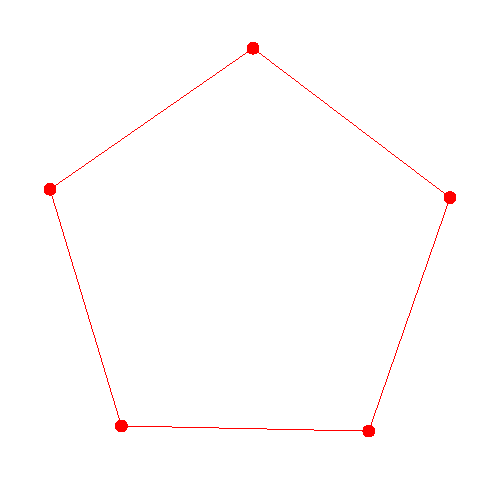
\includegraphics[width=0.4\textwidth]{C5.pdf}}}\caption{This is how you put in a caption for an image.}\label{picture}
\end{figure} 

\section{Theorem Environments}

\begin{theorem}[Ramsey, 1930] \ This is how you create a theorem. The reference next to the Theorem name can be left out.  \label{theorem1}
\end{theorem}

\begin{proof} \ This is how you can create a proof environment.  \end{proof}

In the tex file, note that a label was added within the above theorem environment.  This is so that you can refer to Theorem \ref{theorem1} and if you add more theorems to the paper, they will automatically be renumbered.  The same is true for references.  You may refer to \cite{R}.  It may be necessary to compile the tex file twice before the labels show up.  All sources used in your paper should be listed as in the samples below.  The first, second, and fifth references are articles, while the third and fourth are books.

Here is a sample of a math environment: $\sqrt[4]{14}$.  Use double $\$$ if you wish to have a math environment centered on a line by itself:
$$\mathop{\int}\limits_{1}^{\infty} e^{-x} \ dx.$$
If you would like to have an equation be numbered, use the following:
\begin{equation}  4x^5+3y^7=85. \label{eq} \end{equation}
You can then refer label in the equation.  Eg., equation (\ref{eq}) pulls up the correct number.

Equations, inequalities, etc... can be aligned using the following commands:
\begin{align} \delta (H) &= n-(r-1)-\Delta (\overline{H}) \notag \\
                                    &\ge n-(r-1)-(m+2) \notag \\
                                    &\ge n-m-r-1 \label{ineq} \end{align}
As with the equation environment, each line that has $\backslash$notag will not be labelled, and putting a label allows you to refer to property (\ref{ineq}).

Matrices can be created using the array command:

$$\left( \begin{array}{rrr} -2 & 3 & -7 \\ 2 & 0 & 4 \end{array} \right)$$
% Note that the 3 r's after the above array command right-align the entries.  Replacing any of them with l or c will left-align or center the corresponding columns.

\bibliographystyle{amsplain}
\begin{thebibliography}{10}

\bibitem{C} V. Chv\'atal, {\it Tree-complete Graph Ramsey Numbers,}  J. Graph Theory {\bf 1} (1977), 93.

\bibitem{CH} V. Chv\'atal and F. Harary, {\it Generalized Ramsey Theory for Graphs III. Small Off-diagonal Numbers,} Pacific J. Math. {\bf 41} (1972), 335-345.

\bibitem{IR} K. Ireland and M. Rosen, ``A Classical
Introduction to Modern Number Theory,'' $2^{nd}$ edition,
Springer-Verlag, 1990.

\bibitem{J} G. Janusz, ``Algebraic Number Fields,'' $2^{nd}$ edition, Graduate Studies in Mathematics {\bf 7}, American Mathematical Society, Providence, RI, 1996.

\bibitem{R} F. Ramsey, {\it On a Problem of Formal Logic,} Proc. London Math. Soc. {\bf 30} (1930), 264-286.



\end{thebibliography}


\end{document}
